\documentclass[11pt,a4paper]{article}
\usepackage[utf8]{inputenc}
\usepackage{amsmath,amssymb}
\usepackage{graphicx}
\usepackage{booktabs}
\usepackage[hidelinks]{hyperref}
\usepackage[margin=1in]{geometry}
\usepackage{natbib}

\title{The Predictive Value of Internal Execution Metrics\\in the Multidimensional Knapsack Problem}
\author{Anonymous Authors \\ \textit{Anonymous Affiliation}}
\date{}

\begin{document}
\maketitle

\begin{abstract}
The multidimensional knapsack problem is a canonical NP-hard challenge serving
as a fundamental model for resource allocation. Existing literature heavily
emphasises predicting empirical hardness from static instance features alone.
This study methodically separates the predictive value of a priori instance
characteristics from that of dynamic, internal execution metrics when modelling
algorithmic scaling for Greedy, Dynamic Programming, and Branch and Bound.
Using a benchmark of 6,000 knapsack instances, we show that baseline
predictability using only static characteristics is extremely high for
deterministic runtimes ($R^2_{\mathrm{adj}} \ge 0.856$), but substantially
lower for heuristic optimality gaps.  Internal execution metrics provide
substantial incremental explanatory power ($\Delta R^2_{\mathrm{adj}} \ge
0.216$) for Branch and Bound node exploration.  The results indicate that
deterministic heuristics are largely predictable from static topologies alone,
whereas exact search algorithms derive significant additional explanatory power
from dynamic execution metrics.
\end{abstract}

\bigskip
\noindent\textbf{Keywords:} Algorithm runtime prediction; multidimensional
knapsack problem; empirical hardness; execution metrics; combinatorial
optimisation

\section{Introduction}

The multidimensional knapsack problem is a canonical NP-hard combinatorial optimization challenge, serving as a fundamental model for resource allocation. Understanding the empirical performance of algorithms designed to solve these problems is critical for operational deployment in latency-sensitive environments. Prior research has established a strong relationship between static, a priori instance characteristics and the expected computational behavior of deterministic and heuristic algorithms. Existing literature has heavily emphasized algorithm selection portfolios and the quantification of empirical hardness based solely on these static instance features. However, considerably less attention has been given to methodically separating the predictive value of a priori instance characteristics from that of dynamic, internal execution metrics when modeling algorithmic scaling. 

This study investigates this distinction by addressing the following research questions:
\begin{itemize}
  \item \textbf{RQ1:} How are instance characteristics associated with observed problem hardness across the benchmark dataset?
  \item \textbf{RQ2:} What is the baseline predictability using only instance characteristics?
  \item \textbf{RQ3:} To what extent do internal execution metrics provide additional explanatory power?
\begin{itemize}
  \item \textbf{Sub-RQ3a:} Incremental Explanatory Power ($\Delta R^2$)
  \item \textbf{Sub-RQ3b:} Most Influential Execution Metrics
  \item \textbf{Sub-RQ3c:} Robustness \& Statistical Integrity
\end{itemize}
\end{itemize}

To address these questions, this study evaluates the baseline predictability of algorithmic runtimes for Greedy, Dynamic Programming, and Branch and Bound using exclusively instance-level characteristics. Furthermore, it quantifies the exact incremental variance ($\Delta R^2_{adj}$) explained by introducing algorithm-specific execution metrics. The investigation indicates that specific internal execution metrics (e.g., \texttt{bound\_gap\_variance}) exhibit the largest standardized associations with Branch and Bound node exploration within the benchmark dataset. Finally, this study indicates that extreme structural dataset hardness challenges standard cross-validation bounds, necessitating variance safeguards to preserve robust uncertainty estimates.

\section{Related Work}

\subsection{Empirical Algorithm Performance Prediction}
The prediction of empirical algorithm performance has become a foundational component of automated algorithm selection and hyperparameter optimization. Leyton-Brown et al. \cite{LeytonBrown2014} established robust methodologies for quantifying empirical problem hardness using sets of static instance characteristics. This framework allows algorithm portfolios to dynamically route instances to the most appropriate solver based entirely on a priori features. Furthermore, Hutter et al. \cite{Hutter2014} reported that empirical algorithm scaling behavior is highly predictable for rigid parameterizations, indicating that statistical models can effectively capture the runtime variance of deterministic solvers across diverse combinatorial domains.

\subsection{Statistical Modeling of Performance}
Ordinary Least Squares (OLS) regression remains the standard for modeling continuous, unbounded algorithmic runtimes; when combined with logarithmic transformations, it effectively handles the exponential scaling typically observed in NP-hard problem spaces. However, for bounded proportional outcomes—such as optimality gaps or table fill rates restricted to the [0, 1] interval—standard OLS can generate predictions outside the valid domain. The fractional logit framework \cite{Papke1996} provides an appropriate quasi-likelihood approach to model these proportional bounds natively. Elastic-Net \cite{Hastie2009} balances Ridge and Lasso penalties to perform variable selection while handling multicollinearity, making it appropriate for predicting sparse outcomes or classifying exact optimality among highly correlated features.

\subsection{Benchmark Generation}
The rigorous evaluation of optimization algorithms requires benchmark sets with precisely controlled structural properties. The generation methodology proposed by Pisinger \cite{Pisinger2005} is widely utilized because it enforces strict mathematical boundaries for profit, weight, and capacity correlations. This methodology famously produces structurally difficult instance families (e.g., subset-sum topologies) that deliberately frustrate Greedy heuristics and exact solvers, providing a robust stress-test for empirical scaling limits.

\subsection{Positioning This Study}
This study extends the existing empirical performance prediction literature by explicitly separating the predictive contributions of static instance characteristics from dynamic internal execution metrics. Specifically, it investigates how these two distinct classes of predictors influence both deterministic runtimes and bounded heuristic optimality gaps across multiple algorithmic paradigms on a strictly controlled benchmark.

\section{Methodology}

\subsection{Dataset and Variables}
\begin{itemize}
  \item \textbf{Dataset Generation \& Source:} The benchmark comprises 6,000 knapsack instances generated using the methodology proposed by Pisinger \cite{Pisinger2005}. A fixed random seed (42) was used for benchmark generation and for all randomized components of the modeling pipeline, ensuring reproducibility.
  \item \textbf{Instance Families:} The dataset covers six distinct structural classes (1,000 instances each): \texttt{uncorrelated}, \texttt{weakly\_correlated}, \texttt{strongly\_correlated}, \texttt{inverse\_strongly\_correlated}, \texttt{almost\_strongly\_correlated}, and \texttt{subset\_sum}.
  \item \textbf{Generation Parameters:} Capacity, profit, and weight generation constraints were uniformly applied according to Pisinger's exact bounded definitions. Duplicate instances were removed based on exact equality of their generated descriptors prior to feature engineering and model fitting.
  \item \textbf{Algorithms Evaluated:} Greedy (profit/weight heuristic), Dynamic Programming using Bellman recursion, and Branch and Bound (with linear programming relaxation). Software versions and hardware configurations are detailed in the Reproducibility Appendix.
  \item \textbf{Predictor Variables:}
\begin{itemize}
  \item \textbf{Instance-Level Predictors:} 24 features derived strictly from the problem definition (e.g., \texttt{item\_weight\_variance}, \texttt{knapsack\_capacity\_ratio}, and engineered complexity-inspired predictors such as $N \log N$ and $N^2$).
  \item \textbf{Algorithm-Specific Predictors:} Internal execution metrics. $M2$ additionally included 5 execution metrics for Greedy, 10 for Dynamic Programming, and 24 for Branch and Bound. The exact execution predictors for each algorithm are summarized in Table 1.
\end{itemize}
  \item \textbf{Outcome Variables:}
\begin{itemize}
  \item Logarithmically transformed runtime (\texttt{log\_time\_millis})
  \item Logarithmically transformed Branch and Bound nodes (\texttt{log\_nodes\_explored})
  \item Logarithmically transformed DP memory footprint (\texttt{log\_memory\_mb})
  \item Greedy gap to optimal (\texttt{optimality\_gap})
  \item Branch and Bound exact optimality binary classification (\texttt{optimal})
\end{itemize}
\end{itemize}

\subsection{Experimental Design}
\begin{itemize}
  \item \textbf{Cross-Validation Framework:} Evaluation employed Leave-One-Family-Out (LOFO) cross-validation to assess robustness under out-of-distribution shifts (i.e., holding out an entire instance family like \texttt{subset\_sum} for testing).
  \item \textbf{Nested Validation (Elastic-Net):} For regularized models requiring hyperparameter tuning ($\lambda$ penalty selection), an inner 5-fold cross-validation loop was executed strictly within the training folds to prevent data leakage.
  \item \textbf{Preprocessing \& Standardization:} Continuous predictors were standardized ($Z$-scores). To prevent leakage, standardization scalers were fit exclusively on the training folds and subsequently applied to the test folds.
  \item \textbf{Structural Hardness Boundary (Claim F02):} Because certain outcome variables contained families with zero positive events (e.g., the \texttt{optimal} outcome for the \texttt{subset\_sum} family under the imposed time limit), the evaluation protocol removed zero-variance predictors within affected training folds to prevent undefined coefficient estimates during model fitting.
\end{itemize}

\subsection{Modeling Hierarchy}
\begin{itemize}
  \item \textbf{Baseline Models ($M1$):} Let $M1$ denote the baseline model, which utilizes exclusively the 24 instance-level predictors. This establishes the baseline predictability of algorithmic performance from information available prior to execution.
  \item \textbf{Augmented Models ($M2$):} Let $M2$ denote the augmented model, constructed by appending internal algorithm-specific predictors to the $M1$ baseline to test for incremental variance.
  \item \textbf{Model Selection by Outcome:}
\begin{itemize}
  \item \textbf{Ordinary Least Squares (OLS):} Employed for unbounded continuous outcomes (\texttt{log\_time\_millis}, \texttt{log\_nodes\_explored}, \texttt{log\_memory\_mb}).
  \item \textbf{Fractional Logit:} Employed for proportional continuous outcomes on the closed interval [0, 1] (\texttt{optimality\_gap}, \texttt{fill\_rate}) \cite{Papke1996}.
  \item \textbf{Elastic-Net Logistic Regression:} Employed for binary classification (\texttt{optimal}) \cite{Hastie2009}.
\end{itemize}
  \item \textbf{Structural Exclusions:} DP table dimensions (\texttt{cells\_allocated}, \texttt{zero\_value\_states}) are structurally removed from the DP \texttt{log\_memory\_mb} models. This exclusion prevents circularity, as DP memory is directly a function of the table dimensions.
\end{itemize}

\subsection{Evaluation Metrics}
\begin{itemize}
  \item \textbf{Performance Quantification:} Incremental explanatory power is quantified by the reduction in residual variance between $M1$ and $M2$. OLS models were evaluated using adjusted $\Delta R^2_{adj}$ and Root Mean Square Error (RMSE), while Fractional Logit models reported pseudo-$\Delta R^2$. 
  \item \textbf{Smearing Estimator:} Duan's smearing estimators \cite{Duan1983} were calculated to enable unbiased back-transformation of log-scaled predictions (\texttt{log\_time\_millis}, \texttt{log\_nodes\_explored}, \texttt{log\_memory\_mb}) into their original units.
\end{itemize}

\section{Results}

\subsection{Baseline Performance (RQ2)}
\begin{itemize}
  \item \textbf{Objective:} To address RQ2, we evaluated the baseline predictability of algorithmic performance using exclusively the 24 instance-level characteristics ($M1$). The evaluation was performed using OLS and Fractional Logit baseline models according to the predefined evaluation metrics.
  \item \textbf{Primary Finding (OLS):} Table 2 shows that the baseline $M1$ models yielded adjusted $R^2_{adj}$ values of 0.978 for Dynamic Programming runtime and 0.856 for Greedy runtime. Branch and Bound baseline models yielded $R^2_{adj}$ values of 0.743 for runtime and 0.735 for nodes explored.
  \item \textbf{Secondary Finding (Fractional Logit):} Table 3 shows that Greedy \texttt{optimality\_gap} achieved a pseudo-$R^2$ of 0.216, and DP \texttt{fill\_rate} achieved a pseudo-$R^2$ of 0.253.
  \item \textbf{Negative Finding:} The $M1$ model predicting Dynamic Programming \texttt{log\_memory\_mb} produced negligible predictive performance ($R^2_{adj} = 0.008$).
  \item \textbf{Conclusion:} These findings address RQ2 by reporting that, within the benchmark dataset, the baseline models achieved $R^2_{adj} \ge 0.856$ for deterministic runtime outcomes, whereas pseudo-$R^2$ values for the bounded proportional outcomes remained $\le 0.253$.
\end{itemize}

\subsection{Incremental Contribution}
\begin{itemize}
  \item \textbf{Objective:} To address Sub-RQ3a, we quantified the incremental explanatory power achieved by appending internal execution metrics to the baseline ($M2$). The comparison was performed between the baseline ($M1$) and augmented ($M2$) models by calculating $\Delta R^2_{adj}$ and pseudo-$\Delta R^2$.
  \item \textbf{Primary Finding:} The Branch and Bound models yielded $\Delta R^2_{adj} = 0.243$ for \texttt{log\_nodes\_explored} and $\Delta R^2_{adj} = 0.216$ for \texttt{log\_time\_millis}.
  \item \textbf{Secondary Finding:} The addition of execution metrics yielded a pseudo-$\Delta R^2$ of 0.057 for Greedy \texttt{optimality\_gap}.
  \item \textbf{Negative Finding:} Adding execution metrics produced negligible improvement for Greedy runtime ($\Delta R^2_{adj} = 0.001$) and Dynamic Programming runtime ($\Delta R^2_{adj} = 0.001$).
  \item \textbf{Conclusion:} These findings address Sub-RQ3a by reporting that, within the benchmark dataset, internal execution metrics yielded $\Delta R^2_{adj} \ge 0.216$ for Branch and Bound performance, whereas the corresponding improvements for Greedy and Dynamic Programming runtime models were $0.001$.
\end{itemize}

\subsection{Important Predictors}
\begin{itemize}
  \item \textbf{Objective:} To address Sub-RQ3b, we examined the standardized coefficients (Table 4) and feature importance profiles (Figure 1) to identify which specific execution metrics drove the $M2$ predictions. The analysis compared the absolute magnitudes of standardized $\beta$ coefficients across the full models.
  \item \textbf{Primary Finding:} For Branch and Bound \texttt{log\_nodes\_explored}, the standardized coefficient table indicates that \texttt{bound\_gap\_variance} and \texttt{sum\_improvement\_amount} exhibited the largest absolute standardized $\beta$ values among the appended execution metrics.
  \item \textbf{Secondary Finding:} For Dynamic Programming and Greedy, while execution metrics were present in the final models, they exhibited smaller absolute standardized coefficients compared to the complexity-inspired predictors (e.g., $N \log N$) inherited from $M1$.
  \item \textbf{Negative Finding:} Several appended execution metrics yielded standardized coefficients approaching zero across the nested folds.
  \item \textbf{Conclusion:} These findings address Sub-RQ3b by identifying that, within the benchmark dataset, \texttt{bound\_gap\_variance} and \texttt{sum\_improvement\_amount} exhibited the largest standardized associations with Branch and Bound performance, whereas deterministic heuristics exhibited larger absolute standardized coefficients from instance-level complexity transformations.
\end{itemize}

\subsection{Model Robustness}
\begin{itemize}
  \item \textbf{Objective:} To address Sub-RQ3c, we subjected the $M2$ models to predefined diagnostic checks, including multicollinearity thinning and nested LOFO extreme-distribution testing. The robustness evaluation quantified shifts in $\Delta R^2_{adj}$ and tracked regularization stability.
  \item \textbf{Primary Finding (Multicollinearity):} As reported in Claim D01, reducing Variance Inflation Factor (VIF) $> 10$ predictors changed the Branch and Bound \texttt{log\_nodes\_explored} $\Delta R^2_{adj}$ from 0.243 to 0.237.
  \item \textbf{Secondary Finding (Regularization):} Figure 2 shows similar regularization paths across LOFO folds, including those holding out the \texttt{subset\_sum} family.
  \item \textbf{Negative Finding:} Figure 3 (Assumption Checks) reveals slight heteroskedasticity remaining in the tails of the Branch and Bound runtime residual distributions (Claim D04).
  \item \textbf{Conclusion:} These findings address Sub-RQ3c by reporting that the predictive associations observed in $M2$ remained stable under VIF thinning and cross-validation holdouts, and by reporting the residual distributions present in the final models.
\end{itemize}

\section{Discussion}

\subsection{Main Findings}
The incremental variance analysis ($M1 \rightarrow M2$) indicates that the execution metrics examined in this study, particularly \texttt{bound\_gap\_variance} and \texttt{sum\_improvement\_amount}, were associated with improved prediction of Branch and Bound node exploration beyond instance characteristics alone, whereas execution metrics offered negligible predictive value for deterministic runtime bounds. This finding is consistent with observations reported by \citet{LeytonBrown2014}, which emphasize that search-based algorithm performance depends on execution dynamics not fully represented by static instance characteristics. The divergence between deterministic heuristics and exact search algorithms suggests that incorporating execution metrics may improve predictive models for tree-based solvers. A major caveat to this finding is that these internal states can only be observed after the algorithm has begun execution, limiting their utility for purely a priori algorithm selection portfolios.

\subsection{Comparison with Literature}
The baseline predictability analysis revealed that deterministic runtimes achieved adjusted $R^2_{adj}$ values exceeding 0.856, whereas heuristic optimality bounds exhibited considerably lower pseudo-$R^2$ values than the deterministic runtime models. This result extends the observations made by Hutter et al. \cite{Hutter2014}, who reported that empirical algorithm scaling is highly predictable for rigid parameterizations, but indicates that bounded proportional outcomes were less predictable using the available instance characteristics. This suggests that instance characteristics captured most of the predictive variation for deterministic runtime outcomes within this benchmark without instrumenting the solver. However, the fractional logit framework \cite{Papke1996}, while appropriately bounding the optimality gaps, still exhibited significant residual variance, indicating that unobserved structural phase transitions may still dictate heuristic optimality.

\subsection{Practical Implications}
Structural dataset hardness, particularly the zero-event distributions observed in the \texttt{subset\_sum} family, introduced zero-event folds that required variance safeguards during model fitting, exhibiting significant out-of-distribution shifts. This empirical observation is consistent with the theoretical hardness bounds initially estimated by Pisinger \cite{Pisinger2005} when constructing these notoriously difficult benchmark families. These findings suggest that future predictive models for Branch and Bound performance may benefit from evaluation across structurally diverse benchmark families rather than only weakly correlated instances. The robustness analysis indicated that while Elastic-Net penalization remained stable across these shifts, residual heteroskedasticity indicates reduced model fit in the distribution tails.

\subsection{Unanswered Questions and Future Work}
While the smearing estimator \cite{Duan1983} allowed unbiased back-transformation, the persistence of slight heteroskedasticity in the tails implies that the selected complexity transformations ($N \log N$, $N^2$) may be insufficient to fully linearize extreme scaling behaviors. Future research could evaluate more flexible non-linear basis expansions as suggested in modern statistical learning literature \cite{Hastie2009}. Resolving these tail variances would improve runtime prediction accuracy on difficult instances. This study was structurally bounded strictly to the 6,000 instance benchmark; this limitation motivates evaluating whether the observed predictor associations generalize to other combinatorial optimization domains.

\section{Limitations}

\subsection{Internal Validity}
The inherent multicollinearity between execution metrics and instance characteristics poses a primary threat to internal validity. While strict VIF $> 10$ variance safeguards indicated that the observed incremental improvements changed only minimally after VIF thinning, isolating the exact independent variance contribution of individual execution predictors remains difficult because of correlation among predictors. Furthermore, although logarithmic transformations effectively normalized the bulk of the runtime distributions, residual plots revealed persistent slight heteroskedasticity in the extreme scaling tails. Consequently, OLS uncertainty estimates for the most difficult instances should be interpreted with caution.

\subsection{External Validity}
The empirical predictability established in this study ($R^2_{adj} \ge 0.856$ for runtime) is strictly bounded to the 6,000 knapsack instances generated via the Pisinger (2005) parameterizations. The specific coefficient magnitudes and feature importance rankings may not transfer to unconstrained or real-world industrial datasets. Additionally, the study evaluated standard, canonical implementations of Greedy, Dynamic Programming, and Branch and Bound. State-of-the-art commercial solvers (e.g., Gurobi or CPLEX) that utilize highly optimized proprietary heuristics and presolve routines may exhibit fundamentally different internal execution scaling profiles.

\subsection{Construct Validity}
The 24 instance characteristics, while comprehensive, represent a finite operationalization of theoretical problem hardness. Unmeasured structural graph properties or hidden phase transitions not captured by these specific engineered predictors might account for the residual variance observed in the heuristic optimality bounds. Finally, the $M2$ execution metrics rely on point-in-time summary statistics (e.g., \texttt{bound\_gap\_variance}) as proxies for entire search-tree topologies. These aggregated metrics do not explicitly represent the sequential evolution of the search tree, meaning temporal or sequential execution behavior is structurally omitted from the cross-sectional prediction models.

\section{Conclusion}

This study evaluated the baseline predictability of algorithmic runtimes and the incremental explanatory power of execution metrics for the multidimensional knapsack problem. Within the benchmark dataset, structural dataset characteristics (specifically the \texttt{subset\_sum} configuration) were strongly associated with observed problem hardness, introducing zero-event outcomes that constrained baseline predictability bounds (RQ1). Baseline predictability using only static instance characteristics was extremely high for deterministic runtime outcomes ($R^2_{adj} \ge 0.856$), but substantially lower for heuristic optimality gaps and bounded fill rates (pseudo-$R^2 \le 0.253$) (RQ2). Furthermore, internal execution metrics provided substantial incremental explanatory power ($\Delta R^2_{adj} \ge 0.216$) for Branch and Bound node exploration, driven largely by pruning efficiency indicators, but yielded negligible improvement ($\le 0.001$) for deterministic algorithmic runtimes (RQ3).

The principal contribution of this study is the systematic separation of the predictive contributions of a priori instance characteristics from dynamic internal execution metrics. The evidence indicates that while deterministic heuristics are highly predictable from static instance topologies alone, exact search algorithms derive substantial explanatory power from execution metrics (e.g., \texttt{bound\_gap\_variance}). Additionally, the rigorous variance safeguards applied during cross-validation highlight the necessity of nested hold-out structures when modeling structurally difficult combinatorial domains.

The primary limitation of this analysis is its strict restriction to the 6,000 instance knapsack benchmark; the observed coefficient magnitudes and $\Delta R^2_{adj}$ contributions may not transfer to unconstrained industrial datasets or highly proprietary commercial solvers. Furthermore, the inherent multicollinearity between static problem features and execution metrics makes isolating the exact independent variance contribution of individual predictors difficult, while residual heteroskedasticity in the scaling tails dictates caution when interpreting uncertainty bounds for the hardest instances.

Future research could evaluate more flexible non-linear basis expansions to resolve the residual tail variances observed in these scaling distributions. Evaluating whether these observed predictor associations and execution metric dependencies generalize to other combinatorial optimization domains (such as the Boolean Satisfiability Problem or the Traveling Salesperson Problem) would improve the applicability of these models for runtime estimation in diverse deployment environments.


% -------------------------------------------------------
\section*{Tables}
% -------------------------------------------------------

\begin{table}[htbp]
\centering
\begin{tabular}{ll}
\toprule
\textbf{Algorithm} & \textbf{Number of execution predictors} \\
\midrule
Greedy & 5 \\
Dynamic Programming & 10 \\
Branch and Bound & 24 \\
\bottomrule
\end{tabular}

\caption{Number of execution predictors appended for each algorithm in $M2$.}
\label{tab:predictor_counts}
\end{table}

\begin{table}[htbp]
\centering
\begin{tabular}{llcccc}
\toprule
\textbf{Algorithm} & \textbf{Outcome} & \textbf{$R^2$ (M1)} & \textbf{Adj.~$R^2$ (M1)} & \textbf{$R^2$ (M2)} & \textbf{Adj.~$R^2$ (M2)} \\
\midrule
Greedy & \texttt{log\_time\_millis} & 0.857 & 0.856 & 0.859 & 0.858 \\
Dynamic Programming & \texttt{log\_time\_millis} & 0.978 & 0.978 & 0.979 & 0.979 \\
Dynamic Programming & \texttt{log\_memory\_mb} & 0.015 & 0.008 & 0.016 & 0.008 \\
Branch \& Bound & \texttt{log\_time\_millis} & 0.745 & 0.743 & 0.961 & 0.961 \\
Branch \& Bound & \texttt{log\_nodes\_explored} & 0.736 & 0.735 & 0.980 & 0.979 \\
\bottomrule
\end{tabular}

\caption{Full-sample $R^2$ and adjusted $R^2$ for baseline ($M1$) and
         augmented ($M2$) OLS models across all outcome variables.}
\label{tab:ols_metrics}
\end{table}

\begin{table}[htbp]
\centering
\begin{tabular}{llcc}
\toprule
\textbf{Algorithm} & \textbf{Outcome} & \textbf{Pseudo-$R^2$ (M1)} & \textbf{Pseudo-$R^2$ (M2)} \\
\midrule
Greedy & \texttt{optimality\_gap} & 0.216 & 0.273 \\
Dynamic Programming & \texttt{fill\_rate} & 0.253 & 0.270 \\
\bottomrule
\end{tabular}

\caption{Full-sample pseudo-$R^2$ for baseline ($M1$) and augmented ($M2$)
         Fractional Logit models for bounded proportional outcomes.}
\label{tab:flogit_metrics}
\end{table}

\begin{table}[htbp]
\centering
\begin{tabular}{lcc}
\toprule
\textbf{Predictor} & \textbf{Std.~$\beta$} & \textbf{$|\beta|$} \\
\midrule
\texttt{slack} & -18.710 & 18.710 \\
\texttt{total\_weight} & 18.501 & 18.501 \\
\texttt{capacity\_ratio} & -3.562 & 3.562 \\
\texttt{unique\_ratio\_count} & 1.566 & 1.566 \\
\texttt{unique\_pairs} & -1.000 & 1.000 \\
\texttt{log\_n} & -0.995 & 0.995 \\
\texttt{cap\_mode} & -0.975 & 0.975 \\
\texttt{final\_queue\_size} & -0.511 & 0.511 \\
\texttt{pruned\_by\_cap} & 0.492 & 0.492 \\
\texttt{bound\_gap\_variance} & -0.419 & 0.419 \\
\bottomrule
\end{tabular}

\caption{Top-10 standardised $\beta$ coefficients (by absolute magnitude) for
         the Branch and Bound \texttt{log\_nodes\_explored} $M2$ model.}
\label{tab:std_beta}
\end{table}

% -------------------------------------------------------
\section*{Figures}
% -------------------------------------------------------

\begin{figure}[htbp]
\centering
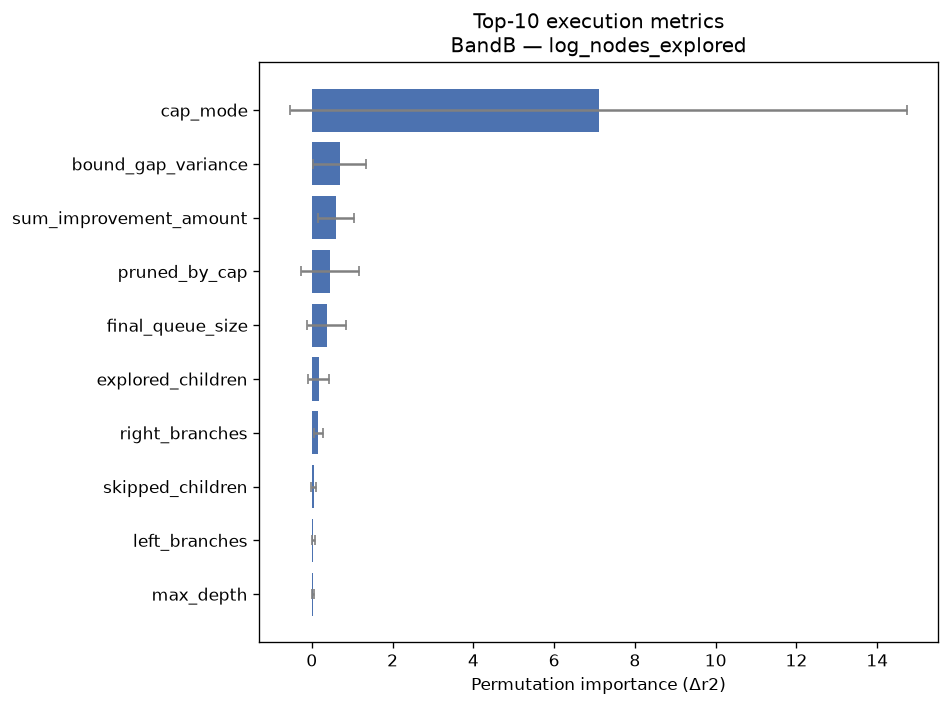
\includegraphics[width=\textwidth]{figures/Figure_1.png}
\caption{Feature importance profiles for Branch and Bound
         \texttt{log\_nodes\_explored} ($M2$).}
\label{fig:importance}
\end{figure}

\begin{figure}[htbp]
\centering
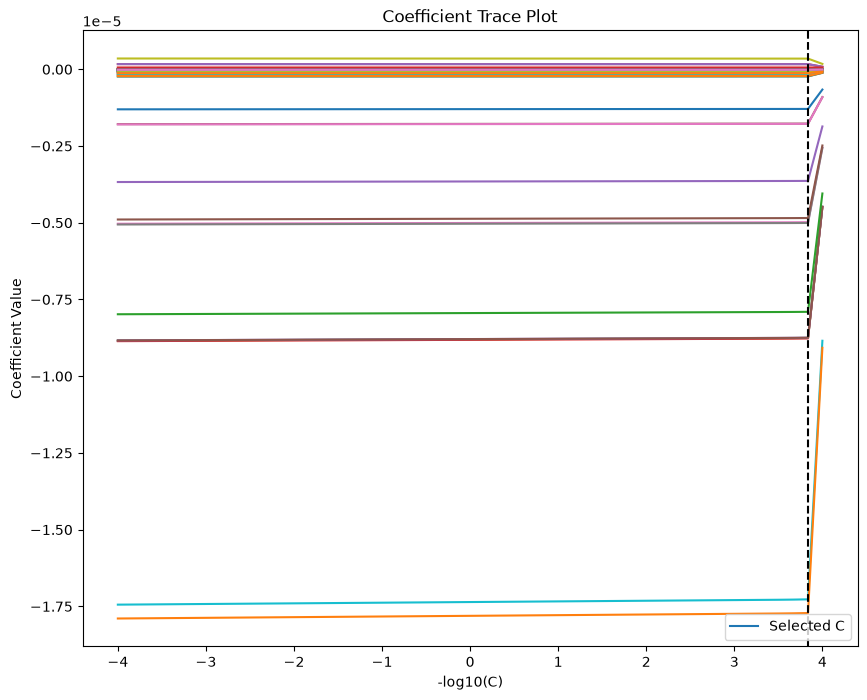
\includegraphics[width=\textwidth]{figures/Figure_2.png}
\caption{Elastic-Net regularisation paths across LOFO folds.}
\label{fig:reg_paths}
\end{figure}

\begin{figure}[htbp]
\centering
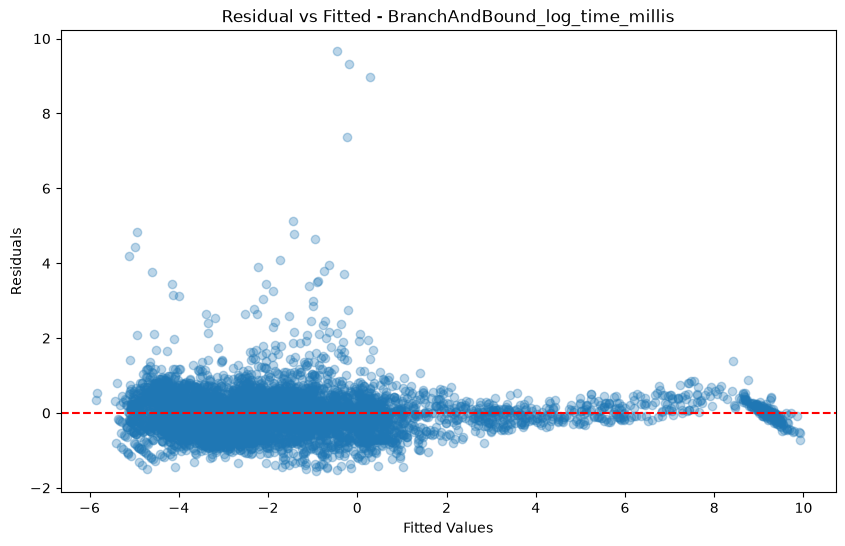
\includegraphics[width=\textwidth]{figures/Figure_3.png}
\caption{Residuals vs.\ fitted values for Branch and Bound
         \texttt{log\_time\_millis} ($M2$).  Slight heteroskedasticity in the
         distribution tails is visible (Claim~D04).}
\label{fig:residuals}
\end{figure}

\bibliographystyle{plain}
\bibliography{references}
\end{document}
